\documentclass{article}

\usepackage{longtable}
\usepackage{fancyhdr}
\usepackage{booktabs}
\usepackage{rotating}
\usepackage{graphicx}
\usepackage{multicol}

\title{\textbf{\LaTeX\ Report}}
\date{\textbf{U.R.N-1805158}}
\author{\textbf{Aman Chauhan}}
\pagestyle{fancy}
\fancyhf{}
\lhead{Latex}
\rhead{Report}
\rfoot{Page \thepage}

\begin{document}

\maketitle
\newpage
\title{\underline{ABSTRACT}}
\paragraph{In this report you will get basic knowledge about latex. Latex is used by scientific and academic communities for writing journal etc, which may or may not contain mathematical formulas or other complex notation. Latex is a typesetting language which is used to to make reports in text which can further converted into pdf form. Latex uses many different text formats in order to decorate our text which looks good in report. Latex is also helpful in order to write mathametical notations and expressions as it as we write in notebook by pen.The best thing about this report is that this report is also written in latex.It is the best example to show the usage of latex. }
\newpage

\section{Introduction}
Creating documents with \LaTeX\ is simple. In contrast to Word, you start off with a plain       text file (.tex file) which contains LaTeX code and the actual content (i.e. text). LaTeX 	uses control statements, which define how your content should be formatted. Before you 			can see what the final result looks like, the LaTeX compiler will take your .tex file and 	compile it into a pdf file.
	
\section{Sections And Paragraph}
We can easily make sections and sub-sections in our report in order to make table of 			content in our report.We can do this by using commands:\\
\textbf{section\{\}}\\
\textbf{subsection\{\}}\\
\textbf{subsubsection\{\}}\\\\
Also we use paragraphs and sub-paragraphs in our report by using commands:\\
\textbf{paragraph\{\}}\\
\textbf{subparagraph\{\}}
	
\section{Header And Footer}
Also, we can use headers and footers in our report.Header is used to show which chapter 		number is going and it also shows name of the chapter.Footer is helpful to show page 			numbering.
There is a package named fancyhdr which can be included as: usepackage\{fancyhdr\}\\\\
After the package was included we can easily create headers and footers.With 					\textbf{rfoot} command right footer is written and with \textbf{lfoot} command left 			footer is 						written.Similalry,With \textbf{rhead} command right 			header is written and with \textbf{lhead} command 		left header is written.

\newpage

\section{Bold Italic Underline}
This feature can be used to distinguish the text in our report.If we want to highlight our text then we can use this feature.\\\\
1.For bold,command is \textbf{textbf}\\
Example :- \textbf{This text is bold.}\\\\
2.For italic,command is \textbf{textit}\\
Example :- \textit{This text is italic.}\\\\
3.For underline,command is \underline{underline}\\
Example :- \underline{This text is underlined.}

\section{Spacing}
For adding spaces in text we use spacing in latex.\\
If we want horizontal space then use "hspace" command. Example :-\\
This is \hspace{1cm}text.\\
In above example space between "is" and "text" is 1cm.\\\\
Similarly, if we want vertical space in two lines then use "vspace" command. Example :-\\
This is line 1.
	
\vspace{1cm}

This is line 2.\\
In above example space between line 1 and 2 is 1 cm.\\\\
If we want to fill horizontal space and vertical space then command is \textbf{hfill} and 	\textbf{vfill}. Example :\\
This is \hfill text.\\
Start of line.
\vfill
End of page.

\newpage

\section{Images}
From time to time, it's necessary to add pictures to your documents. Using LaTeX all pictures will be indexed automatically and tagged with successive numbers when using the \textbf{graphicx} package.
\begin{center}
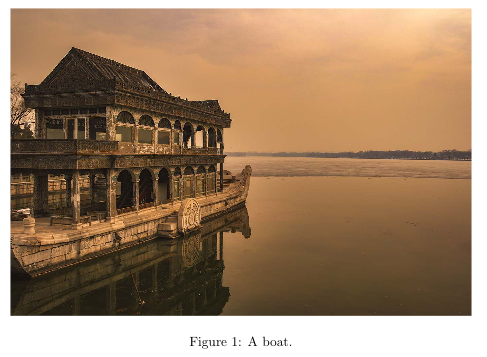
\includegraphics[width=5cm,height=4cm]{boat.png}
\end{center}
If you want to add multi pictures in a row then you have to use two include commands.
\begin{center}
	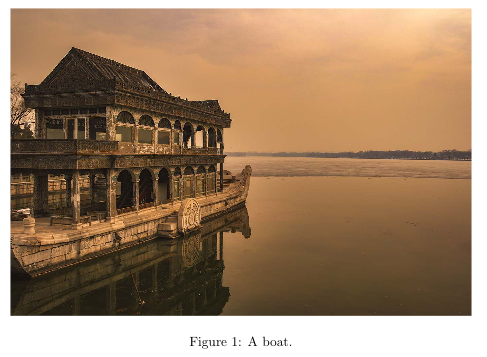
\includegraphics[width=5cm,height=4cm]{boat.png}
	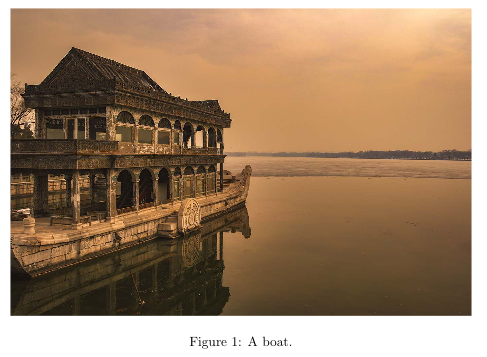
\includegraphics[width=5cm,height=4cm]{boat.png}
\end{center}
For using images with text we can simply use multi column commands.\\

\begin{center}
\begin{multicols}{2}
Here is an example of text with image.This can be done using \textbf{multicol} commands.

\columnbreak

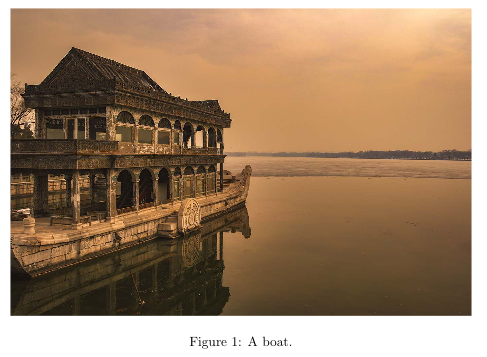
\includegraphics[width=\linewidth]{boat.png}
  
\end{multicols}
\end{center}

\begin{center}
\begin{multicols}{2}
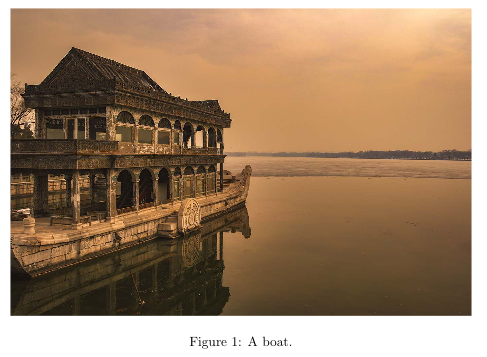
\includegraphics[width=\linewidth]{boat.png}

\columnbreak

Similarly if we want picture in left and text in right then this can also be done easily.
  
\end{multicols}
\end{center}

\section{Tables}
In this we're going to learn how to use the table and tabular environments to create tables in LaTeX.Tables are very useful in order to maintain data in report.Table is written inside the table environment.Here is an example of simple table:

\begin{table}[h!]
  \begin{center}
    \caption{Your first table.}
    \label{tab:table1}
    \begin{tabular}{l|c|r}
      \textbf{Value 1} & \textbf{Value 2} & \textbf{Value 3}\\
      $\alpha$ & $\beta$ & $\gamma$ \\
      \hline
      1 & 1110.1 & a\\
      2 & 10.1 & b\\
      3 & 23.113231 & c\\
    \end{tabular}
  \end{center}
\end{table}

\subsection{Prettier tables with booktabs}
Of course beauty is always in the eye of the beholder, but I personally think, that the default \textbf{hlines} used by the table environment are not very pretty. For my tables, i always use the \textbf{booktabs} package, which provides much prettier horizontal separators and the usage is not harder compared to simply using hlines.\\
After using package named \textbf{booktabs} we can easily use commands of that package.There are commands like: \textbf{toprule},\textbf{midrule} and \textbf{bottomrule}.Example is given as: 
\newpage
\begin{table}[h!]
  \begin{center}
    \caption{Table using booktabs.}
    \label{tab:table1}
    \begin{tabular}{c|c|c}
      \toprule
      \textbf{Value 1} & \textbf{Value 2} & \textbf{Value 3}\\
      $\alpha$ & $\beta$ & $\gamma$ \\
      \midrule
      1 & 1110.1 & a\\
      2 & 10.1 & b\\
      3 & 23.113231 & c\\
      \bottomrule
    \end{tabular}
  \end{center}
\end{table}

\subsection{Multipage Table}
If you have a lot of rows in your table, you will notice that by default, the table will be cropped at the bottom of the page, which is certainly not what you want. The package longtable provides a convenient way, to make tables span multiple pages. Of course we have to add the package to our preamble before we can start using it. For multipage you have to include  \textbf{longtable}.

\begin{longtable}{c|c|c}
  \caption{Multipage table.}
  \label{tab:table1}\\
  \toprule
  \textbf{Value 1} & \textbf{Value 2} & \textbf{Value 3}\\
  $\alpha$ & $\beta$ & $\gamma$ \\
  \midrule
  \endfirsthead
  \toprule
  \textbf{Value 1} & \textbf{Value 2} & \textbf{Value 3}\\
  $\alpha$ & $\beta$ & $\gamma$ \\
  \midrule
  \endhead
  1 & 1110.1    & a\\
  2 & 10.1      & b\\
  3 & 23.113231 & c\\
  4 & 54.458    & d\\
  ..& ..........&..\\
  ..& ..........&..\\
  ..& ..........&..\\
  ..& ..........&..\\
  ..& ..........&..\\
  ..& ..........&..\\
  ..& ..........&..\\
  ..& ..........&..\\
  ..& ..........&..\\
  ..& ..........&..\\
  ..& ..........&..\\
  ..& ..........&..\\
  ..& ..........&..\\
  ..& ..........&..\\
  ..& ..........&..\\
  ..& ..........&..\\
  ..& ..........&..\\
  ..& ..........&..\\
  ..& ..........&..\\
  ..& ..........&..\\
  ..& ..........&..\\
  ..& ..........&..\\
  ..& ..........&..\\
  ..& ..........&..\\
  ..& ..........&..\\
  ..& ..........&..\\
  ..& ..........&..\\
  ..& ..........&..\\
  ..& ..........&..\\
  ..& ..........&..\\
  ..& ..........&..\\
  ..& ..........&..\\
  ..& ..........&..\\
  ..& ..........&..\\
  ..& ..........&..\\
  ..& ..........&..\\
  ..& ..........&..\\
  ..& ..........&..\\
  ..& ..........&..\\
  ..& ..........&..\\
  ..& ..........&..\\
  ..& ..........&..\\
  26& 42.4586   &z\\
  
  \bottomrule
\end{longtable}

\subsection{Sideways Table}
If we want a ratated table in our report, we also done this by simply using package \textbf{rotating}.\\
This package provides the sidewaystable environment, which is very easy to use. Just replace the table environment with the sidewaystable environment .\\
Example is given as:

\begin{sidewaystable}[h!]
  \begin{center}
  \caption{Landscape table.}
  \label{tab:table1}
  \begin{tabular}{c|c|c}
  	\toprule
  	\textbf{Value 1} & \textbf{Value 2} & \textbf{Value 3}\\
  	$\alpha$ & $\beta$ & $\gamma$ \\
    \midrule
    1 & 1110.1 & a\\
    2 & 10.1 & b\\
    3 & 23.113231 & c\\
    \bottomrule
  \end{tabular}
  \end{center}
\end{sidewaystable}

\newpage
\newpage
\begin{thebibliography}{9}
\bibitem{link0} 
Google
\\\texttt{https://google.com}

\bibitem{link1} 
\LaTeX\
\\\texttt{https://www.latex-tutorial.com/tutorials/}
 
\bibitem{knuthwebsite} 
Overleaf
\\\texttt{https://www.overleaf.com/learn/latex/Tutorials}
\end{thebibliography}

\end{document}
